\section{Marketing and Sales}
Market adoption and sales are the true measures of success. Clearly convey your strategy and tactics to penetrate the market and drive sales. Potential investors want to understand your customer awareness and buying stimulus programs from the customer�s and salesperson�s perspective. If you are not currently selling your product, explain your product launch plans. Convince the audience that you have an effective go-to-market strategy that will not break the bank.

Include the following key points:
- What is your go-to-market strategy?
- How will you drive market demand for your product?
- What is your branding strategy?
- What is your pricing strategy?
- What is your marketing communication plan?
- How will you recruit and build your sales force?
- What is your distribution plan?
- Who will be your key partners?
- What is your customer retention strategy?
- Who are your largest customers?

Refer to the information you have documented in Market Strategy Development Workbook 2: Critical Value Factors and Market Strategy Development Workbook 3: Strategic Marketing Approach.

Describe your go-to-market strategy in the corresponding section of the Business Planning and Executive Summary workbook template. Use the information from the Market Strategy Development workbook guides that is indicated in the bullet list above.



\subsection{The Competition}
To properly evaluate the competition and find our foothold in the market, table \ref{competition} shows our competition profile based on the EERC framework.

\begin{table}[ht]
\caption{Defining the Competition} % title of Table
\centering % used for centering table
\begin{tabular}{| c c c |} % centered columns (4 columns)
\hline
Compeitor & Type of Competition & Strengths \\
\hline % inserts single horizontal line
Previously established approval software contracts. & Economic & Strength: Our product will be easier to justify using in their current budgets.\\ % inserting body of the table space
Document revision control schemes (ie: Google Docs) & Direct & Strength: Our product will focus specifically on the professional challenges associated with establishing a secure approval process. \\
\hline %inserts single line
\end{tabular}
\label{competition} % is used to refer this table in the text
\end{table}

\subsection{How we Differ from the Competition}
We focus on differentiating ourselves from our competitors by providing a product that helps develop a productive and frustration-free work environment. Seeking approval for your work by a higher-up should not be a cumbersome process. Acknowledgements allows users to quickly draft an approval request and send it off in minutes from anywhere. 

Every aspect of our software will focus on helping the customer have a hassle-free experience. The interface will be uncluttered and easy to use. Mobile and desktop web applications will allow for your Acknowledgements account to be easily accessible. Finally, our eager team will be available to help create custom functionality to serve the ever-changing needs of our clients.

Our value curve shows visually how we differentiatie ourselves from our competition.

\begin{figure}[ht!]
\centering
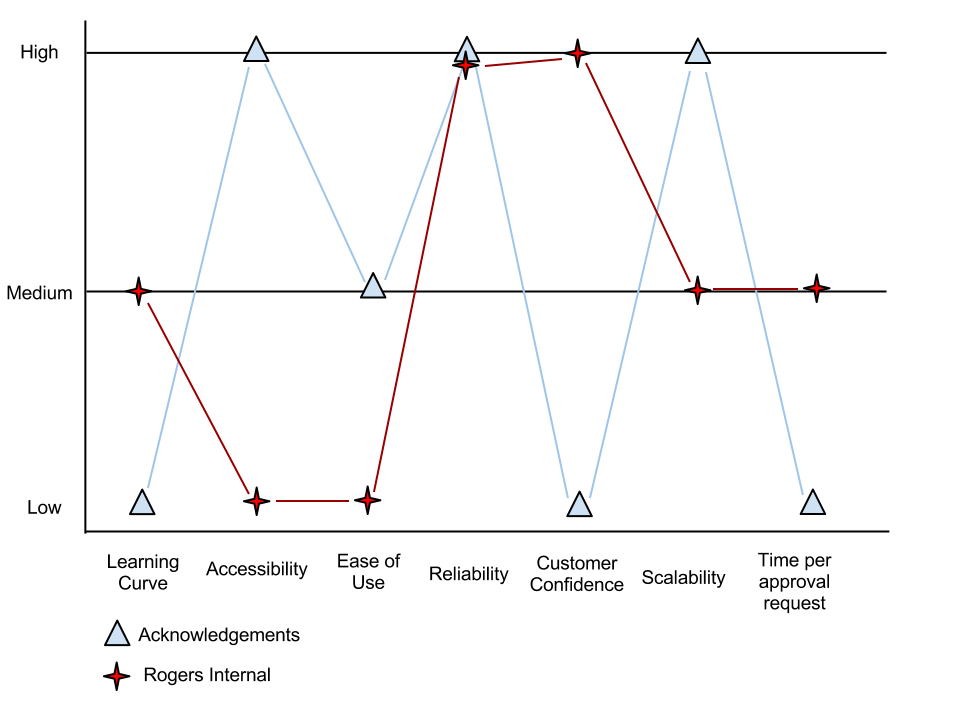
\includegraphics[width=150mm]{images/MSCI454-ValueCurve.png}
\caption{Value Curve}
\label{valuecurve}
\end{figure}

\subsection{Go-to-Market Strategy}